\documentclass[twoside]{book}

% Packages required by doxygen
\usepackage{fixltx2e}
\usepackage{calc}
\usepackage{doxygen}
\usepackage[export]{adjustbox} % also loads graphicx
\usepackage{graphicx}
\usepackage[utf8]{inputenc}
\usepackage{makeidx}
\usepackage{multicol}
\usepackage{multirow}
\PassOptionsToPackage{warn}{textcomp}
\usepackage{textcomp}
\usepackage[nointegrals]{wasysym}
\usepackage[table]{xcolor}

% Font selection
\usepackage[T1]{fontenc}
\usepackage[scaled=.90]{helvet}
\usepackage{courier}
\usepackage{amssymb}
\usepackage{sectsty}
\renewcommand{\familydefault}{\sfdefault}
\allsectionsfont{%
  \fontseries{bc}\selectfont%
  \color{darkgray}%
}
\renewcommand{\DoxyLabelFont}{%
  \fontseries{bc}\selectfont%
  \color{darkgray}%
}
\newcommand{\+}{\discretionary{\mbox{\scriptsize$\hookleftarrow$}}{}{}}

% Page & text layout
\usepackage{geometry}
\geometry{%
  a4paper,%
  top=2.5cm,%
  bottom=2.5cm,%
  left=2.5cm,%
  right=2.5cm%
}
\tolerance=750
\hfuzz=15pt
\hbadness=750
\setlength{\emergencystretch}{15pt}
\setlength{\parindent}{0cm}
\setlength{\parskip}{3ex plus 2ex minus 2ex}
\makeatletter
\renewcommand{\paragraph}{%
  \@startsection{paragraph}{4}{0ex}{-1.0ex}{1.0ex}{%
    \normalfont\normalsize\bfseries\SS@parafont%
  }%
}
\renewcommand{\subparagraph}{%
  \@startsection{subparagraph}{5}{0ex}{-1.0ex}{1.0ex}{%
    \normalfont\normalsize\bfseries\SS@subparafont%
  }%
}
\makeatother

% Headers & footers
\usepackage{fancyhdr}
\pagestyle{fancyplain}
\fancyhead[LE]{\fancyplain{}{\bfseries\thepage}}
\fancyhead[CE]{\fancyplain{}{}}
\fancyhead[RE]{\fancyplain{}{\bfseries\leftmark}}
\fancyhead[LO]{\fancyplain{}{\bfseries\rightmark}}
\fancyhead[CO]{\fancyplain{}{}}
\fancyhead[RO]{\fancyplain{}{\bfseries\thepage}}
\fancyfoot[LE]{\fancyplain{}{}}
\fancyfoot[CE]{\fancyplain{}{}}
\fancyfoot[RE]{\fancyplain{}{\bfseries\scriptsize Generated by Doxygen }}
\fancyfoot[LO]{\fancyplain{}{\bfseries\scriptsize Generated by Doxygen }}
\fancyfoot[CO]{\fancyplain{}{}}
\fancyfoot[RO]{\fancyplain{}{}}
\renewcommand{\footrulewidth}{0.4pt}
\renewcommand{\chaptermark}[1]{%
  \markboth{#1}{}%
}
\renewcommand{\sectionmark}[1]{%
  \markright{\thesection\ #1}%
}

% Indices & bibliography
\usepackage{natbib}
\usepackage[titles]{tocloft}
\setcounter{tocdepth}{3}
\setcounter{secnumdepth}{5}
\makeindex

% Hyperlinks (required, but should be loaded last)
\usepackage{ifpdf}
\ifpdf
  \usepackage[pdftex,pagebackref=true]{hyperref}
\else
  \usepackage[ps2pdf,pagebackref=true]{hyperref}
\fi
\hypersetup{%
  colorlinks=true,%
  linkcolor=blue,%
  citecolor=blue,%
  unicode%
}

% Custom commands
\newcommand{\clearemptydoublepage}{%
  \newpage{\pagestyle{empty}\cleardoublepage}%
}

\usepackage{caption}
\captionsetup{labelsep=space,justification=centering,font={bf},singlelinecheck=off,skip=4pt,position=top}

%===== C O N T E N T S =====

\begin{document}

% Titlepage & ToC
\hypersetup{pageanchor=false,
             bookmarksnumbered=true,
             pdfencoding=unicode
            }
\pagenumbering{alph}
\begin{titlepage}
\vspace*{7cm}
\begin{center}%
{\Large Dieu\+Khien\+Nhac\+Nuoc }\\
\vspace*{1cm}
{\large Generated by Doxygen 1.8.14}\\
\end{center}
\end{titlepage}
\clearemptydoublepage
\pagenumbering{roman}
\tableofcontents
\clearemptydoublepage
\pagenumbering{arabic}
\hypersetup{pageanchor=true}

%--- Begin generated contents ---
\chapter{Hierarchical Index}
\section{Class Hierarchy}
This inheritance list is sorted roughly, but not completely, alphabetically\+:\begin{DoxyCompactList}
\item \contentsline{section}{Music\+Presenter\+Item}{\pageref{struct_music_presenter_item}}{}
\item \contentsline{section}{Presenter\+Frame}{\pageref{struct_presenter_frame}}{}
\item \contentsline{section}{Previous\+Frame}{\pageref{struct_previous_frame}}{}
\item Q\+Abstract\+List\+Model\begin{DoxyCompactList}
\item \contentsline{section}{Music\+Presenter\+Model}{\pageref{class_music_presenter_model}}{}
\item \contentsline{section}{time\+Slot\+Model}{\pageref{classtime_slot_model}}{}
\end{DoxyCompactList}
\item Q\+Object\begin{DoxyCompactList}
\item \contentsline{section}{Music\+Presenter\+List}{\pageref{class_music_presenter_list}}{}
\item \contentsline{section}{Presenter\+Frame\+List}{\pageref{class_presenter_frame_list}}{}
\item \contentsline{section}{the\+Interface\+God}{\pageref{classthe_interface_god}}{}
\item \contentsline{section}{time\+Slot\+List}{\pageref{classtime_slot_list}}{}
\end{DoxyCompactList}
\item \contentsline{section}{qt\+\_\+meta\+\_\+stringdata\+\_\+\+Music\+Presenter\+Element\+\_\+t}{\pageref{structqt__meta__stringdata___music_presenter_element__t}}{}
\item \contentsline{section}{qt\+\_\+meta\+\_\+stringdata\+\_\+\+Music\+Presenter\+List\+\_\+t}{\pageref{structqt__meta__stringdata___music_presenter_list__t}}{}
\item \contentsline{section}{qt\+\_\+meta\+\_\+stringdata\+\_\+\+Music\+Presenter\+Model\+\_\+t}{\pageref{structqt__meta__stringdata___music_presenter_model__t}}{}
\item \contentsline{section}{qt\+\_\+meta\+\_\+stringdata\+\_\+\+Presenter\+Frame\+List\+\_\+t}{\pageref{structqt__meta__stringdata___presenter_frame_list__t}}{}
\item \contentsline{section}{qt\+\_\+meta\+\_\+stringdata\+\_\+the\+Interface\+God\+\_\+t}{\pageref{structqt__meta__stringdata__the_interface_god__t}}{}
\item \contentsline{section}{qt\+\_\+meta\+\_\+stringdata\+\_\+time\+Slot\+List\+\_\+t}{\pageref{structqt__meta__stringdata__time_slot_list__t}}{}
\item \contentsline{section}{qt\+\_\+meta\+\_\+stringdata\+\_\+time\+Slot\+Model\+\_\+t}{\pageref{structqt__meta__stringdata__time_slot_model__t}}{}
\item \contentsline{section}{time\+Slot}{\pageref{classtime_slot}}{}
\item \contentsline{section}{time\+Slot\+Item}{\pageref{structtime_slot_item}}{}
\end{DoxyCompactList}

\chapter{Class Index}
\section{Class List}
Here are the classes, structs, unions and interfaces with brief descriptions\+:\begin{DoxyCompactList}
\item\contentsline{section}{\mbox{\hyperlink{struct_music_presenter_item}{Music\+Presenter\+Item}} }{\pageref{struct_music_presenter_item}}{}
\item\contentsline{section}{\mbox{\hyperlink{class_music_presenter_list}{Music\+Presenter\+List}} }{\pageref{class_music_presenter_list}}{}
\item\contentsline{section}{\mbox{\hyperlink{class_music_presenter_model}{Music\+Presenter\+Model}} }{\pageref{class_music_presenter_model}}{}
\item\contentsline{section}{\mbox{\hyperlink{struct_presenter_frame}{Presenter\+Frame}} }{\pageref{struct_presenter_frame}}{}
\item\contentsline{section}{\mbox{\hyperlink{class_presenter_frame_list}{Presenter\+Frame\+List}} }{\pageref{class_presenter_frame_list}}{}
\item\contentsline{section}{\mbox{\hyperlink{struct_previous_frame}{Previous\+Frame}} }{\pageref{struct_previous_frame}}{}
\item\contentsline{section}{\mbox{\hyperlink{structqt__meta__stringdata___music_presenter_element__t}{qt\+\_\+meta\+\_\+stringdata\+\_\+\+Music\+Presenter\+Element\+\_\+t}} }{\pageref{structqt__meta__stringdata___music_presenter_element__t}}{}
\item\contentsline{section}{\mbox{\hyperlink{structqt__meta__stringdata___music_presenter_list__t}{qt\+\_\+meta\+\_\+stringdata\+\_\+\+Music\+Presenter\+List\+\_\+t}} }{\pageref{structqt__meta__stringdata___music_presenter_list__t}}{}
\item\contentsline{section}{\mbox{\hyperlink{structqt__meta__stringdata___music_presenter_model__t}{qt\+\_\+meta\+\_\+stringdata\+\_\+\+Music\+Presenter\+Model\+\_\+t}} }{\pageref{structqt__meta__stringdata___music_presenter_model__t}}{}
\item\contentsline{section}{\mbox{\hyperlink{structqt__meta__stringdata___presenter_frame_list__t}{qt\+\_\+meta\+\_\+stringdata\+\_\+\+Presenter\+Frame\+List\+\_\+t}} }{\pageref{structqt__meta__stringdata___presenter_frame_list__t}}{}
\item\contentsline{section}{\mbox{\hyperlink{structqt__meta__stringdata__the_interface_god__t}{qt\+\_\+meta\+\_\+stringdata\+\_\+the\+Interface\+God\+\_\+t}} }{\pageref{structqt__meta__stringdata__the_interface_god__t}}{}
\item\contentsline{section}{\mbox{\hyperlink{structqt__meta__stringdata__time_slot_list__t}{qt\+\_\+meta\+\_\+stringdata\+\_\+time\+Slot\+List\+\_\+t}} }{\pageref{structqt__meta__stringdata__time_slot_list__t}}{}
\item\contentsline{section}{\mbox{\hyperlink{structqt__meta__stringdata__time_slot_model__t}{qt\+\_\+meta\+\_\+stringdata\+\_\+time\+Slot\+Model\+\_\+t}} }{\pageref{structqt__meta__stringdata__time_slot_model__t}}{}
\item\contentsline{section}{\mbox{\hyperlink{classthe_interface_god}{the\+Interface\+God}} }{\pageref{classthe_interface_god}}{}
\item\contentsline{section}{\mbox{\hyperlink{classtime_slot}{time\+Slot}} }{\pageref{classtime_slot}}{}
\item\contentsline{section}{\mbox{\hyperlink{structtime_slot_item}{time\+Slot\+Item}} }{\pageref{structtime_slot_item}}{}
\item\contentsline{section}{\mbox{\hyperlink{classtime_slot_list}{time\+Slot\+List}} }{\pageref{classtime_slot_list}}{}
\item\contentsline{section}{\mbox{\hyperlink{classtime_slot_model}{time\+Slot\+Model}} }{\pageref{classtime_slot_model}}{}
\end{DoxyCompactList}

\chapter{Class Documentation}
\hypertarget{struct_music_presenter_item}{}\section{Music\+Presenter\+Item Struct Reference}
\label{struct_music_presenter_item}\index{Music\+Presenter\+Item@{Music\+Presenter\+Item}}
\subsection*{Public Attributes}
\begin{DoxyCompactItemize}
\item 
\mbox{\Hypertarget{struct_music_presenter_item_aedd277faf798664e15e7ed25d31f8c28}\label{struct_music_presenter_item_aedd277faf798664e15e7ed25d31f8c28}} 
int {\bfseries id}
\item 
\mbox{\Hypertarget{struct_music_presenter_item_a731da3c2eb3657a7c32ab332928392c8}\label{struct_music_presenter_item_a731da3c2eb3657a7c32ab332928392c8}} 
quint8 {\bfseries group}
\item 
\mbox{\Hypertarget{struct_music_presenter_item_ae777fd26d47640ca3625da3c43c3646b}\label{struct_music_presenter_item_ae777fd26d47640ca3625da3c43c3646b}} 
bool {\bfseries Valve\+On\+Off}
\item 
\mbox{\Hypertarget{struct_music_presenter_item_a612270b7dfd0a735f2c82806ab988966}\label{struct_music_presenter_item_a612270b7dfd0a735f2c82806ab988966}} 
bool {\bfseries Led\+On\+Off}
\item 
\mbox{\Hypertarget{struct_music_presenter_item_a44ae461c82d448f1de13f10ba97807c3}\label{struct_music_presenter_item_a44ae461c82d448f1de13f10ba97807c3}} 
bool {\bfseries Inverter}
\item 
\mbox{\Hypertarget{struct_music_presenter_item_addc6a7753cd0992ecdd1f625d7f9900e}\label{struct_music_presenter_item_addc6a7753cd0992ecdd1f625d7f9900e}} 
Q\+String {\bfseries Led\+Color}
\item 
\mbox{\Hypertarget{struct_music_presenter_item_a8575d087ae129f8f76528e4a3c8482a9}\label{struct_music_presenter_item_a8575d087ae129f8f76528e4a3c8482a9}} 
quint8 {\bfseries Inverter\+Level}
\item 
\mbox{\Hypertarget{struct_music_presenter_item_a154782edf773c9cad6ed6eea71433ab6}\label{struct_music_presenter_item_a154782edf773c9cad6ed6eea71433ab6}} 
quint8 {\bfseries Led\+Channels}
\item 
\mbox{\Hypertarget{struct_music_presenter_item_a1862de2508b9bf3462199f40d856d4d3}\label{struct_music_presenter_item_a1862de2508b9bf3462199f40d856d4d3}} 
quint8 {\bfseries Valve\+Channels}
\item 
\mbox{\Hypertarget{struct_music_presenter_item_a1893b820d7e1c328e2aa1b00cad375ea}\label{struct_music_presenter_item_a1893b820d7e1c328e2aa1b00cad375ea}} 
int {\bfseries X\+Pos}
\item 
\mbox{\Hypertarget{struct_music_presenter_item_abc1d1f25518a37bafa47998de66f5687}\label{struct_music_presenter_item_abc1d1f25518a37bafa47998de66f5687}} 
int {\bfseries Y\+Pos}
\item 
\mbox{\Hypertarget{struct_music_presenter_item_ad7c0917dbf73ba77551ed0c2f1d5fc1a}\label{struct_music_presenter_item_ad7c0917dbf73ba77551ed0c2f1d5fc1a}} 
bool {\bfseries odd}
\end{DoxyCompactItemize}


\subsection{Detailed Description}


Definition at line 8 of file musicpresenterlist.\+h.



The documentation for this struct was generated from the following file\+:\begin{DoxyCompactItemize}
\item 
musicpresenterlist.\+h\end{DoxyCompactItemize}

\hypertarget{class_music_presenter_list}{}\section{Music\+Presenter\+List Class Reference}
\label{class_music_presenter_list}\index{Music\+Presenter\+List@{Music\+Presenter\+List}}
Inheritance diagram for Music\+Presenter\+List\+:\begin{figure}[H]
\begin{center}
\leavevmode
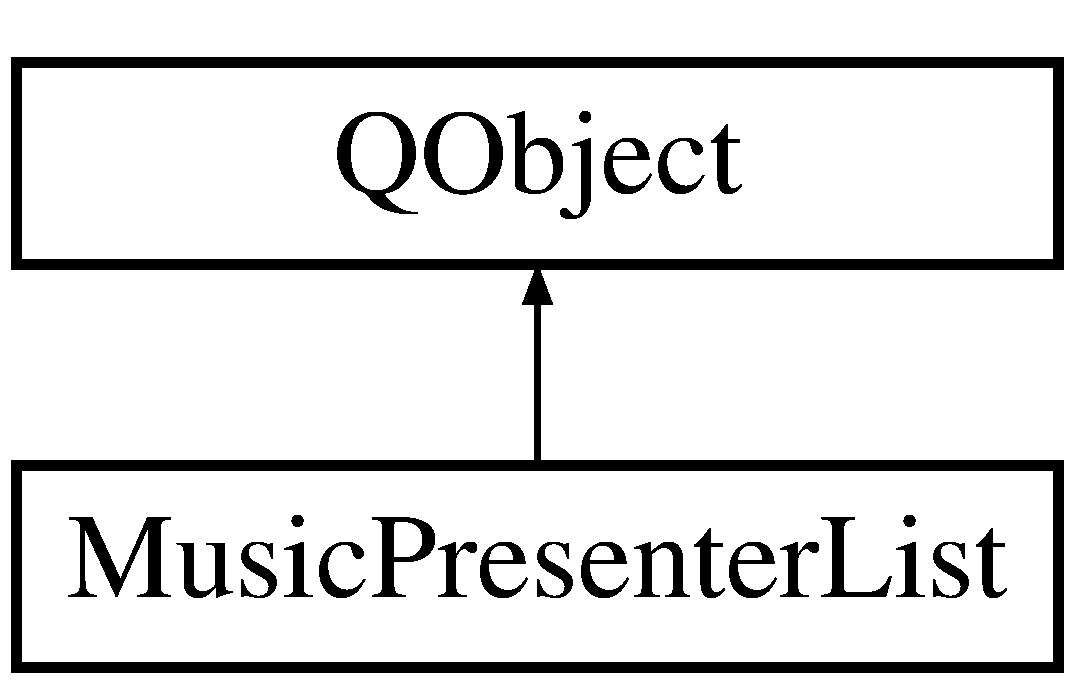
\includegraphics[height=2.000000cm]{class_music_presenter_list}
\end{center}
\end{figure}
\subsection*{Public Slots}
\begin{DoxyCompactItemize}
\item 
\mbox{\Hypertarget{class_music_presenter_list_a9e0f6ae916ed0ed8e357f33e55c22e78}\label{class_music_presenter_list_a9e0f6ae916ed0ed8e357f33e55c22e78}} 
void {\bfseries append\+Item} (const quint8 \&group, int x\+Pos, int y\+Pos)
\item 
\mbox{\Hypertarget{class_music_presenter_list_ae51493321cf61660e3469ed455c618c8}\label{class_music_presenter_list_ae51493321cf61660e3469ed455c618c8}} 
void {\bfseries appen\+Item\+Group6} (bool odd, int x\+Pos, int y\+Pos)
\item 
\mbox{\Hypertarget{class_music_presenter_list_a2686e66f212d6bf3c6f26a49830615c3}\label{class_music_presenter_list_a2686e66f212d6bf3c6f26a49830615c3}} 
void {\bfseries remove\+Items} (const int \&id)
\item 
\mbox{\Hypertarget{class_music_presenter_list_abbc0092ee526cbf9544960b5a63c471d}\label{class_music_presenter_list_abbc0092ee526cbf9544960b5a63c471d}} 
void {\bfseries clear} ()
\item 
\mbox{\Hypertarget{class_music_presenter_list_a5d1cd3b22981c0a9baad72687e6be0c7}\label{class_music_presenter_list_a5d1cd3b22981c0a9baad72687e6be0c7}} 
void {\bfseries frame\+Changed\+Handler} (const \mbox{\hyperlink{struct_presenter_frame}{Presenter\+Frame}} \&frame)
\end{DoxyCompactItemize}
\subsection*{Signals}
\begin{DoxyCompactItemize}
\item 
\mbox{\Hypertarget{class_music_presenter_list_af9065d7835d29c1e95417d1e198f8685}\label{class_music_presenter_list_af9065d7835d29c1e95417d1e198f8685}} 
void {\bfseries pre\+Item\+Appended} ()
\item 
\mbox{\Hypertarget{class_music_presenter_list_a83d746e859bcbe59dec8634b4fc28a62}\label{class_music_presenter_list_a83d746e859bcbe59dec8634b4fc28a62}} 
void {\bfseries post\+Item\+Appended} ()
\item 
\mbox{\Hypertarget{class_music_presenter_list_a8f21f5a1a00c485d015390163bb62243}\label{class_music_presenter_list_a8f21f5a1a00c485d015390163bb62243}} 
void {\bfseries pre\+Item\+Removed} (int index)
\item 
\mbox{\Hypertarget{class_music_presenter_list_aa08884da47905436ecf3cd210863474f}\label{class_music_presenter_list_aa08884da47905436ecf3cd210863474f}} 
void {\bfseries post\+Item\+Removed} ()
\item 
\mbox{\Hypertarget{class_music_presenter_list_a0aa7b8f00f42f011f1236e894c46cd08}\label{class_music_presenter_list_a0aa7b8f00f42f011f1236e894c46cd08}} 
void {\bfseries item\+Changed\+From\+Backend} ()
\end{DoxyCompactItemize}
\subsection*{Public Member Functions}
\begin{DoxyCompactItemize}
\item 
\mbox{\Hypertarget{class_music_presenter_list_a2a4622f9e4f4bfdb8c194ee4658de01f}\label{class_music_presenter_list_a2a4622f9e4f4bfdb8c194ee4658de01f}} 
{\bfseries Music\+Presenter\+List} (Q\+Object $\ast$parent=nullptr)
\item 
\mbox{\Hypertarget{class_music_presenter_list_a683d665dcb75b525ad75ecae2db56bcb}\label{class_music_presenter_list_a683d665dcb75b525ad75ecae2db56bcb}} 
Q\+Vector$<$ \mbox{\hyperlink{struct_music_presenter_item}{Music\+Presenter\+Item}} $>$ {\bfseries items} () const
\item 
\mbox{\Hypertarget{class_music_presenter_list_ac6de919442f269bfd2ce6418950ed5c7}\label{class_music_presenter_list_ac6de919442f269bfd2ce6418950ed5c7}} 
bool {\bfseries set\+Item\+At} (int index, const \mbox{\hyperlink{struct_music_presenter_item}{Music\+Presenter\+Item}} \&item)
\end{DoxyCompactItemize}
\subsection*{Public Attributes}
\begin{DoxyCompactItemize}
\item 
\mbox{\Hypertarget{class_music_presenter_list_af97aa7d1f5d01eb41f7c7b4c9d92e026}\label{class_music_presenter_list_af97aa7d1f5d01eb41f7c7b4c9d92e026}} 
quint8 {\bfseries m\+Group}
\end{DoxyCompactItemize}


\subsection{Detailed Description}


Definition at line 24 of file musicpresenterlist.\+h.



The documentation for this class was generated from the following files\+:\begin{DoxyCompactItemize}
\item 
musicpresenterlist.\+h\item 
debug/moc\+\_\+musicpresenterlist.\+cpp\item 
musicpresenterlist.\+cpp\end{DoxyCompactItemize}

\hypertarget{class_music_presenter_model}{}\section{Music\+Presenter\+Model Class Reference}
\label{class_music_presenter_model}\index{Music\+Presenter\+Model@{Music\+Presenter\+Model}}
Inheritance diagram for Music\+Presenter\+Model\+:\begin{figure}[H]
\begin{center}
\leavevmode
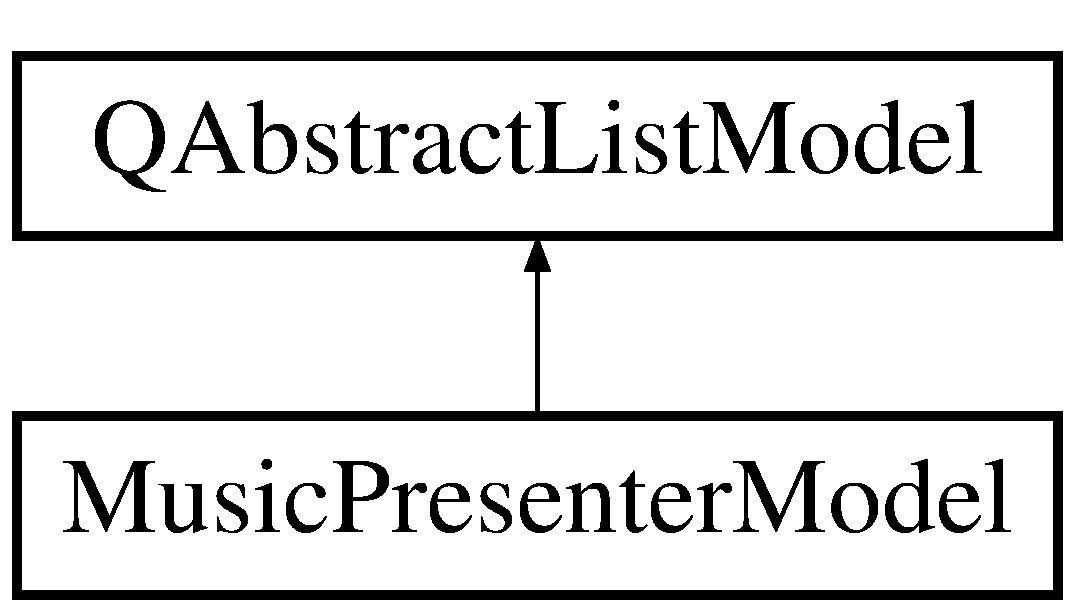
\includegraphics[height=2.000000cm]{class_music_presenter_model}
\end{center}
\end{figure}
\subsection*{Public Types}
\begin{DoxyCompactItemize}
\item 
\mbox{\Hypertarget{class_music_presenter_model_aad086f8b0c5f5a152198fe378eb9d07d}\label{class_music_presenter_model_aad086f8b0c5f5a152198fe378eb9d07d}} 
enum \{ \newline
{\bfseries I\+D\+Role} = Qt\+:\+:User\+Role, 
{\bfseries Group\+Role}, 
{\bfseries Valve\+On\+Off\+Role}, 
{\bfseries Led\+On\+Off\+Role}, 
\newline
{\bfseries Inverter\+Role}, 
{\bfseries Led\+Color\+Role}, 
{\bfseries Inverter\+Level\+Role}, 
{\bfseries L\+E\+D\+Channels\+Role}, 
\newline
{\bfseries Valve\+Channels\+Role}, 
{\bfseries X\+Pos\+Role}, 
{\bfseries Y\+Pos\+Role}, 
{\bfseries Odd\+Role}
 \}
\end{DoxyCompactItemize}
\subsection*{Public Member Functions}
\begin{DoxyCompactItemize}
\item 
\mbox{\Hypertarget{class_music_presenter_model_a361441da604e68b066dbeeda6b349e5f}\label{class_music_presenter_model_a361441da604e68b066dbeeda6b349e5f}} 
{\bfseries Music\+Presenter\+Model} (Q\+Object $\ast$parent=nullptr)
\item 
\mbox{\Hypertarget{class_music_presenter_model_a771f733a651f6a2d91717e5018fbaaa7}\label{class_music_presenter_model_a771f733a651f6a2d91717e5018fbaaa7}} 
int {\bfseries row\+Count} (const Q\+Model\+Index \&parent=Q\+Model\+Index()) const override
\item 
\mbox{\Hypertarget{class_music_presenter_model_a0cb9d531421fde36880d607944dd399b}\label{class_music_presenter_model_a0cb9d531421fde36880d607944dd399b}} 
Q\+Variant {\bfseries data} (const Q\+Model\+Index \&index, int role=Qt\+::\+Display\+Role) const override
\item 
\mbox{\Hypertarget{class_music_presenter_model_ad1ef19cdba7dd3528daa96e85cf510fe}\label{class_music_presenter_model_ad1ef19cdba7dd3528daa96e85cf510fe}} 
bool {\bfseries set\+Data} (const Q\+Model\+Index \&index, const Q\+Variant \&value, int role=Qt\+::\+Edit\+Role) override
\item 
\mbox{\Hypertarget{class_music_presenter_model_accdf24c158fac2167c990920d931d5bb}\label{class_music_presenter_model_accdf24c158fac2167c990920d931d5bb}} 
Qt\+::\+Item\+Flags {\bfseries flags} (const Q\+Model\+Index \&index) const override
\item 
\mbox{\Hypertarget{class_music_presenter_model_a4f0154972fc0cf66972613abc0d056f3}\label{class_music_presenter_model_a4f0154972fc0cf66972613abc0d056f3}} 
virtual Q\+Hash$<$ int, Q\+Byte\+Array $>$ {\bfseries role\+Names} () const override
\item 
\mbox{\Hypertarget{class_music_presenter_model_a516748de38693824273deb3d887c72f6}\label{class_music_presenter_model_a516748de38693824273deb3d887c72f6}} 
\mbox{\hyperlink{class_music_presenter_list}{Music\+Presenter\+List}} $\ast$ {\bfseries list} () const
\item 
\mbox{\Hypertarget{class_music_presenter_model_ab57bce25e4c398f9590e6c9c13dd9ccf}\label{class_music_presenter_model_ab57bce25e4c398f9590e6c9c13dd9ccf}} 
void {\bfseries set\+List} (\mbox{\hyperlink{class_music_presenter_list}{Music\+Presenter\+List}} $\ast$list)
\end{DoxyCompactItemize}
\subsection*{Properties}
\begin{DoxyCompactItemize}
\item 
\mbox{\Hypertarget{class_music_presenter_model_aa39655c9626cd9d1a2eec9adc122918a}\label{class_music_presenter_model_aa39655c9626cd9d1a2eec9adc122918a}} 
\mbox{\hyperlink{class_music_presenter_list}{Music\+Presenter\+List}} {\bfseries list}
\end{DoxyCompactItemize}


\subsection{Detailed Description}


Definition at line 9 of file musicpresentermodel.\+h.



The documentation for this class was generated from the following files\+:\begin{DoxyCompactItemize}
\item 
musicpresentermodel.\+h\item 
musicpresentermodel.\+cpp\end{DoxyCompactItemize}

\hypertarget{struct_presenter_frame}{}\section{Presenter\+Frame Struct Reference}
\label{struct_presenter_frame}\index{Presenter\+Frame@{Presenter\+Frame}}
\subsection*{Public Attributes}
\begin{DoxyCompactItemize}
\item 
\mbox{\Hypertarget{struct_presenter_frame_ab6e74c278ed47206a337946f4285e503}\label{struct_presenter_frame_ab6e74c278ed47206a337946f4285e503}} 
int {\bfseries frame\+No}
\item 
\mbox{\Hypertarget{struct_presenter_frame_a027768e83fa218a53c200ae2cdb818b0}\label{struct_presenter_frame_a027768e83fa218a53c200ae2cdb818b0}} 
bool {\bfseries Inverter}
\item 
\mbox{\Hypertarget{struct_presenter_frame_ae3b6ee796f8b81ac17b9c205b9bededb}\label{struct_presenter_frame_ae3b6ee796f8b81ac17b9c205b9bededb}} 
Q\+List$<$ Q\+String $>$ {\bfseries Led\+Colors}
\item 
\mbox{\Hypertarget{struct_presenter_frame_aae729757acf82d19cef43d6fb393ebfb}\label{struct_presenter_frame_aae729757acf82d19cef43d6fb393ebfb}} 
Q\+List$<$ bool $>$ {\bfseries Valve\+On\+Off}
\item 
\mbox{\Hypertarget{struct_presenter_frame_ab16e28cf8de421804ea8206b87f638f7}\label{struct_presenter_frame_ab16e28cf8de421804ea8206b87f638f7}} 
Q\+List$<$ bool $>$ {\bfseries Led\+On\+Off}
\item 
\mbox{\Hypertarget{struct_presenter_frame_a003a4a04273751f60dd6039965df003b}\label{struct_presenter_frame_a003a4a04273751f60dd6039965df003b}} 
quint8 {\bfseries Inverter\+Level}
\item 
\mbox{\Hypertarget{struct_presenter_frame_afd7452174aa516588265108b958f0310}\label{struct_presenter_frame_afd7452174aa516588265108b958f0310}} 
quint8 {\bfseries Led\+Channels}
\item 
\mbox{\Hypertarget{struct_presenter_frame_abda45e10095e8fd132af2241960ceb84}\label{struct_presenter_frame_abda45e10095e8fd132af2241960ceb84}} 
quint8 {\bfseries Valve\+Channels}
\end{DoxyCompactItemize}


\subsection{Detailed Description}


Definition at line 11 of file presenterframelist.\+h.



The documentation for this struct was generated from the following file\+:\begin{DoxyCompactItemize}
\item 
presenterframelist.\+h\end{DoxyCompactItemize}

\hypertarget{class_presenter_frame_list}{}\section{Presenter\+Frame\+List Class Reference}
\label{class_presenter_frame_list}\index{Presenter\+Frame\+List@{Presenter\+Frame\+List}}
Inheritance diagram for Presenter\+Frame\+List\+:\begin{figure}[H]
\begin{center}
\leavevmode
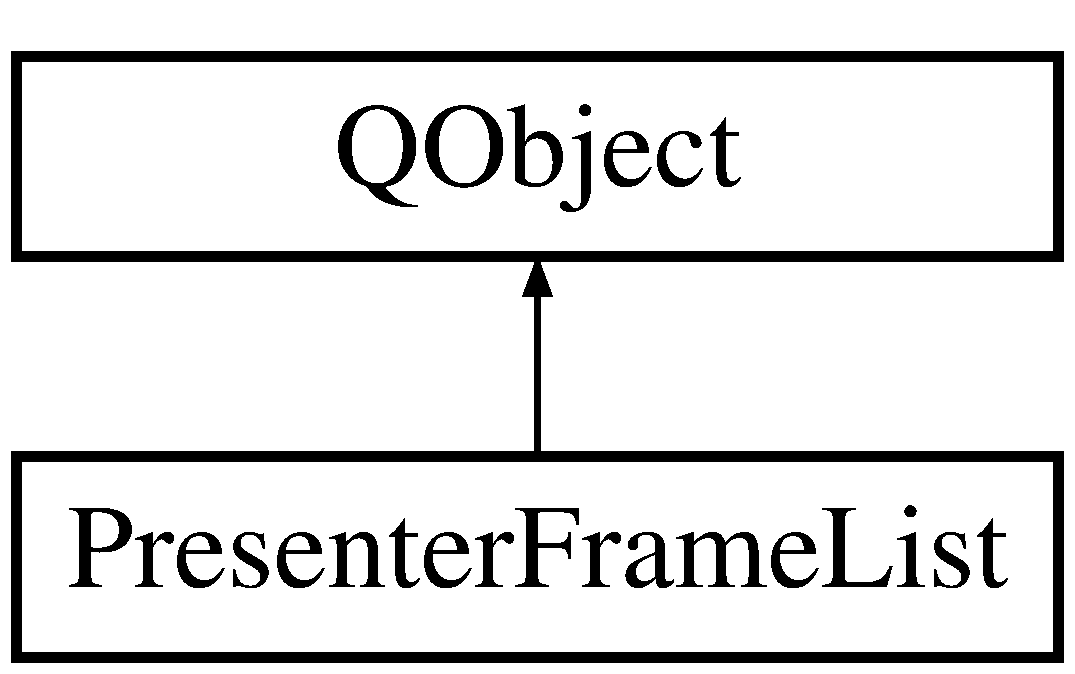
\includegraphics[height=2.000000cm]{class_presenter_frame_list}
\end{center}
\end{figure}
\subsection*{Public Slots}
\begin{DoxyCompactItemize}
\item 
\mbox{\Hypertarget{class_presenter_frame_list_afcddf1fb04e7356b9bae504ed6db9968}\label{class_presenter_frame_list_afcddf1fb04e7356b9bae504ed6db9968}} 
void {\bfseries time\+Slot\+Changed} (const \mbox{\hyperlink{structtime_slot_item}{time\+Slot\+Item}} \&\mbox{\hyperlink{classtime_slot}{time\+Slot}})
\item 
\mbox{\Hypertarget{class_presenter_frame_list_afe96f037c77ac0794e0e59b22736be9e}\label{class_presenter_frame_list_afe96f037c77ac0794e0e59b22736be9e}} 
void {\bfseries time\+Slot\+Removed} (const \mbox{\hyperlink{structtime_slot_item}{time\+Slot\+Item}} \&\mbox{\hyperlink{classtime_slot}{time\+Slot}})
\item 
\mbox{\Hypertarget{class_presenter_frame_list_aaa92436969a77d2a9e4cd176bc3d2978}\label{class_presenter_frame_list_aaa92436969a77d2a9e4cd176bc3d2978}} 
void {\bfseries play\+Frame} (const int \&frame\+No)
\item 
\mbox{\Hypertarget{class_presenter_frame_list_ae304df5f1f1482276d4acead601188df}\label{class_presenter_frame_list_ae304df5f1f1482276d4acead601188df}} 
void {\bfseries regenerate\+Frame\+List} (const int \&Duration, const int \&Frame\+Duration)
\end{DoxyCompactItemize}
\subsection*{Signals}
\begin{DoxyCompactItemize}
\item 
\mbox{\Hypertarget{class_presenter_frame_list_a6429b2e08d2801f3573da06eb9af8ed0}\label{class_presenter_frame_list_a6429b2e08d2801f3573da06eb9af8ed0}} 
void {\bfseries notify\+Frame\+Changed} (const \mbox{\hyperlink{struct_presenter_frame}{Presenter\+Frame}} \&frame)
\end{DoxyCompactItemize}
\subsection*{Public Member Functions}
\begin{DoxyCompactItemize}
\item 
\mbox{\Hypertarget{class_presenter_frame_list_aa2c74556ed2697a6013956973fda6a17}\label{class_presenter_frame_list_aa2c74556ed2697a6013956973fda6a17}} 
{\bfseries Presenter\+Frame\+List} (Q\+Object $\ast$parent=nullptr)
\item 
\mbox{\Hypertarget{class_presenter_frame_list_aa715252ae6dd6bc8dc49aa668eb29748}\label{class_presenter_frame_list_aa715252ae6dd6bc8dc49aa668eb29748}} 
void {\bfseries clear\+List} ()
\item 
\mbox{\Hypertarget{class_presenter_frame_list_a6d446834a3e30812912b730f58ebc89e}\label{class_presenter_frame_list_a6d446834a3e30812912b730f58ebc89e}} 
int {\bfseries get\+Frame\+Duration} () const
\item 
\mbox{\Hypertarget{class_presenter_frame_list_a830ba7bb76301c3755021b3cf33239ab}\label{class_presenter_frame_list_a830ba7bb76301c3755021b3cf33239ab}} 
int {\bfseries get\+Duration} () const
\item 
\mbox{\Hypertarget{class_presenter_frame_list_a8c01086322689b3e14c4f28ecdd7b5fd}\label{class_presenter_frame_list_a8c01086322689b3e14c4f28ecdd7b5fd}} 
int {\bfseries get\+Frame\+No} () const
\item 
\mbox{\Hypertarget{class_presenter_frame_list_a946683cc73234f5c993f5637af5653ff}\label{class_presenter_frame_list_a946683cc73234f5c993f5637af5653ff}} 
\mbox{\hyperlink{struct_presenter_frame}{Presenter\+Frame}} {\bfseries get\+Frame} (const int \&frame\+No)
\item 
\mbox{\Hypertarget{class_presenter_frame_list_a07a924fe311fee3ad0282a95d791e5da}\label{class_presenter_frame_list_a07a924fe311fee3ad0282a95d791e5da}} 
int {\bfseries find\+Frame\+From\+Ms} (const int \&time\+Point)
\end{DoxyCompactItemize}
\subsection*{Public Attributes}
\begin{DoxyCompactItemize}
\item 
\mbox{\Hypertarget{class_presenter_frame_list_ad58bfd5de0cb2df8070dcc17a8d629cf}\label{class_presenter_frame_list_ad58bfd5de0cb2df8070dcc17a8d629cf}} 
int {\bfseries m\+Group}
\end{DoxyCompactItemize}


\subsection{Detailed Description}


Definition at line 29 of file presenterframelist.\+h.



The documentation for this class was generated from the following files\+:\begin{DoxyCompactItemize}
\item 
presenterframelist.\+h\item 
debug/moc\+\_\+presenterframelist.\+cpp\item 
presenterframelist.\+cpp\end{DoxyCompactItemize}

\hypertarget{struct_previous_frame}{}\section{Previous\+Frame Struct Reference}
\label{struct_previous_frame}\index{Previous\+Frame@{Previous\+Frame}}
\subsection*{Public Attributes}
\begin{DoxyCompactItemize}
\item 
\mbox{\Hypertarget{struct_previous_frame_a5a28c233dd3125b595e645898a47a700}\label{struct_previous_frame_a5a28c233dd3125b595e645898a47a700}} 
int {\bfseries id}
\item 
\mbox{\Hypertarget{struct_previous_frame_ae0b9923fb29a6f3c510b934b74cb7770}\label{struct_previous_frame_ae0b9923fb29a6f3c510b934b74cb7770}} 
int {\bfseries From\+Frame}
\item 
\mbox{\Hypertarget{struct_previous_frame_a10b53ca42e0a46671772ca021d05d925}\label{struct_previous_frame_a10b53ca42e0a46671772ca021d05d925}} 
int {\bfseries To\+Frame}
\end{DoxyCompactItemize}


\subsection{Detailed Description}


Definition at line 23 of file presenterframelist.\+h.



The documentation for this struct was generated from the following file\+:\begin{DoxyCompactItemize}
\item 
presenterframelist.\+h\end{DoxyCompactItemize}

\hypertarget{structqt__meta__stringdata___music_presenter_element__t}{}\section{qt\+\_\+meta\+\_\+stringdata\+\_\+\+Music\+Presenter\+Element\+\_\+t Struct Reference}
\label{structqt__meta__stringdata___music_presenter_element__t}\index{qt\+\_\+meta\+\_\+stringdata\+\_\+\+Music\+Presenter\+Element\+\_\+t@{qt\+\_\+meta\+\_\+stringdata\+\_\+\+Music\+Presenter\+Element\+\_\+t}}
\subsection*{Public Attributes}
\begin{DoxyCompactItemize}
\item 
\mbox{\Hypertarget{structqt__meta__stringdata___music_presenter_element__t_a9c2c1cdf376f391fafdb126fb9c656d5}\label{structqt__meta__stringdata___music_presenter_element__t_a9c2c1cdf376f391fafdb126fb9c656d5}} 
Q\+Byte\+Array\+Data {\bfseries data} \mbox{[}1\mbox{]}
\item 
\mbox{\Hypertarget{structqt__meta__stringdata___music_presenter_element__t_a0cb550b2d9807f4d3971bb81dcffefaf}\label{structqt__meta__stringdata___music_presenter_element__t_a0cb550b2d9807f4d3971bb81dcffefaf}} 
char {\bfseries stringdata0} \mbox{[}22\mbox{]}
\end{DoxyCompactItemize}


\subsection{Detailed Description}


Definition at line 23 of file moc\+\_\+musicpresenterelement.\+cpp.



The documentation for this struct was generated from the following file\+:\begin{DoxyCompactItemize}
\item 
debug/moc\+\_\+musicpresenterelement.\+cpp\end{DoxyCompactItemize}

\hypertarget{structqt__meta__stringdata___music_presenter_list__t}{}\section{qt\+\_\+meta\+\_\+stringdata\+\_\+\+Music\+Presenter\+List\+\_\+t Struct Reference}
\label{structqt__meta__stringdata___music_presenter_list__t}\index{qt\+\_\+meta\+\_\+stringdata\+\_\+\+Music\+Presenter\+List\+\_\+t@{qt\+\_\+meta\+\_\+stringdata\+\_\+\+Music\+Presenter\+List\+\_\+t}}
\subsection*{Public Attributes}
\begin{DoxyCompactItemize}
\item 
\mbox{\Hypertarget{structqt__meta__stringdata___music_presenter_list__t_ae345be0e7a0222c3f3f796b873b0b430}\label{structqt__meta__stringdata___music_presenter_list__t_ae345be0e7a0222c3f3f796b873b0b430}} 
Q\+Byte\+Array\+Data {\bfseries data} \mbox{[}20\mbox{]}
\item 
\mbox{\Hypertarget{structqt__meta__stringdata___music_presenter_list__t_acbbe6e51b5fd994e3727f9ae172057ec}\label{structqt__meta__stringdata___music_presenter_list__t_acbbe6e51b5fd994e3727f9ae172057ec}} 
char {\bfseries stringdata0} \mbox{[}222\mbox{]}
\end{DoxyCompactItemize}


\subsection{Detailed Description}


Definition at line 23 of file moc\+\_\+musicpresenterlist.\+cpp.



The documentation for this struct was generated from the following file\+:\begin{DoxyCompactItemize}
\item 
debug/moc\+\_\+musicpresenterlist.\+cpp\end{DoxyCompactItemize}

\hypertarget{structqt__meta__stringdata___music_presenter_model__t}{}\section{qt\+\_\+meta\+\_\+stringdata\+\_\+\+Music\+Presenter\+Model\+\_\+t Struct Reference}
\label{structqt__meta__stringdata___music_presenter_model__t}\index{qt\+\_\+meta\+\_\+stringdata\+\_\+\+Music\+Presenter\+Model\+\_\+t@{qt\+\_\+meta\+\_\+stringdata\+\_\+\+Music\+Presenter\+Model\+\_\+t}}
\subsection*{Public Attributes}
\begin{DoxyCompactItemize}
\item 
\mbox{\Hypertarget{structqt__meta__stringdata___music_presenter_model__t_ac97e066c7c985076c1b76e6f6bbde490}\label{structqt__meta__stringdata___music_presenter_model__t_ac97e066c7c985076c1b76e6f6bbde490}} 
Q\+Byte\+Array\+Data {\bfseries data} \mbox{[}3\mbox{]}
\item 
\mbox{\Hypertarget{structqt__meta__stringdata___music_presenter_model__t_a69fe0ab1bbb8d3fc15641ad7d7900275}\label{structqt__meta__stringdata___music_presenter_model__t_a69fe0ab1bbb8d3fc15641ad7d7900275}} 
char {\bfseries stringdata0} \mbox{[}45\mbox{]}
\end{DoxyCompactItemize}


\subsection{Detailed Description}


Definition at line 23 of file moc\+\_\+musicpresentermodel.\+cpp.



The documentation for this struct was generated from the following file\+:\begin{DoxyCompactItemize}
\item 
debug/moc\+\_\+musicpresentermodel.\+cpp\end{DoxyCompactItemize}

\hypertarget{structqt__meta__stringdata___presenter_frame_list__t}{}\section{qt\+\_\+meta\+\_\+stringdata\+\_\+\+Presenter\+Frame\+List\+\_\+t Struct Reference}
\label{structqt__meta__stringdata___presenter_frame_list__t}\index{qt\+\_\+meta\+\_\+stringdata\+\_\+\+Presenter\+Frame\+List\+\_\+t@{qt\+\_\+meta\+\_\+stringdata\+\_\+\+Presenter\+Frame\+List\+\_\+t}}
\subsection*{Public Attributes}
\begin{DoxyCompactItemize}
\item 
\mbox{\Hypertarget{structqt__meta__stringdata___presenter_frame_list__t_a2be995191a531863c42fe7befc8b8110}\label{structqt__meta__stringdata___presenter_frame_list__t_a2be995191a531863c42fe7befc8b8110}} 
Q\+Byte\+Array\+Data {\bfseries data} \mbox{[}14\mbox{]}
\item 
\mbox{\Hypertarget{structqt__meta__stringdata___presenter_frame_list__t_a4c920b76fca319001c432bd90660044c}\label{structqt__meta__stringdata___presenter_frame_list__t_a4c920b76fca319001c432bd90660044c}} 
char {\bfseries stringdata0} \mbox{[}175\mbox{]}
\end{DoxyCompactItemize}


\subsection{Detailed Description}


Definition at line 23 of file moc\+\_\+presenterframelist.\+cpp.



The documentation for this struct was generated from the following file\+:\begin{DoxyCompactItemize}
\item 
debug/moc\+\_\+presenterframelist.\+cpp\end{DoxyCompactItemize}

\hypertarget{structqt__meta__stringdata__the_interface_god__t}{}\section{qt\+\_\+meta\+\_\+stringdata\+\_\+the\+Interface\+God\+\_\+t Struct Reference}
\label{structqt__meta__stringdata__the_interface_god__t}\index{qt\+\_\+meta\+\_\+stringdata\+\_\+the\+Interface\+God\+\_\+t@{qt\+\_\+meta\+\_\+stringdata\+\_\+the\+Interface\+God\+\_\+t}}
\subsection*{Public Attributes}
\begin{DoxyCompactItemize}
\item 
\mbox{\Hypertarget{structqt__meta__stringdata__the_interface_god__t_af8cd20711806295c9214d366c2e049b1}\label{structqt__meta__stringdata__the_interface_god__t_af8cd20711806295c9214d366c2e049b1}} 
Q\+Byte\+Array\+Data {\bfseries data} \mbox{[}9\mbox{]}
\item 
\mbox{\Hypertarget{structqt__meta__stringdata__the_interface_god__t_a761f62607a4d422abbae792c165f7d0d}\label{structqt__meta__stringdata__the_interface_god__t_a761f62607a4d422abbae792c165f7d0d}} 
char {\bfseries stringdata0} \mbox{[}116\mbox{]}
\end{DoxyCompactItemize}


\subsection{Detailed Description}


Definition at line 23 of file moc\+\_\+theinterfacegod.\+cpp.



The documentation for this struct was generated from the following file\+:\begin{DoxyCompactItemize}
\item 
debug/moc\+\_\+theinterfacegod.\+cpp\end{DoxyCompactItemize}

\hypertarget{structqt__meta__stringdata__time_slot_list__t}{}\section{qt\+\_\+meta\+\_\+stringdata\+\_\+time\+Slot\+List\+\_\+t Struct Reference}
\label{structqt__meta__stringdata__time_slot_list__t}\index{qt\+\_\+meta\+\_\+stringdata\+\_\+time\+Slot\+List\+\_\+t@{qt\+\_\+meta\+\_\+stringdata\+\_\+time\+Slot\+List\+\_\+t}}
\subsection*{Public Attributes}
\begin{DoxyCompactItemize}
\item 
\mbox{\Hypertarget{structqt__meta__stringdata__time_slot_list__t_ac80982dd5282c1d0b48f1bd29a1ed05a}\label{structqt__meta__stringdata__time_slot_list__t_ac80982dd5282c1d0b48f1bd29a1ed05a}} 
Q\+Byte\+Array\+Data {\bfseries data} \mbox{[}21\mbox{]}
\item 
\mbox{\Hypertarget{structqt__meta__stringdata__time_slot_list__t_a0674dd9e6ad5701d5a980de519a04cc8}\label{structqt__meta__stringdata__time_slot_list__t_a0674dd9e6ad5701d5a980de519a04cc8}} 
char {\bfseries stringdata0} \mbox{[}242\mbox{]}
\end{DoxyCompactItemize}


\subsection{Detailed Description}


Definition at line 23 of file moc\+\_\+timeslotlist.\+cpp.



The documentation for this struct was generated from the following file\+:\begin{DoxyCompactItemize}
\item 
debug/moc\+\_\+timeslotlist.\+cpp\end{DoxyCompactItemize}

\hypertarget{structqt__meta__stringdata__time_slot_model__t}{}\section{qt\+\_\+meta\+\_\+stringdata\+\_\+time\+Slot\+Model\+\_\+t Struct Reference}
\label{structqt__meta__stringdata__time_slot_model__t}\index{qt\+\_\+meta\+\_\+stringdata\+\_\+time\+Slot\+Model\+\_\+t@{qt\+\_\+meta\+\_\+stringdata\+\_\+time\+Slot\+Model\+\_\+t}}
\subsection*{Public Attributes}
\begin{DoxyCompactItemize}
\item 
\mbox{\Hypertarget{structqt__meta__stringdata__time_slot_model__t_a81939825efd5726f46d05db0eab55f15}\label{structqt__meta__stringdata__time_slot_model__t_a81939825efd5726f46d05db0eab55f15}} 
Q\+Byte\+Array\+Data {\bfseries data} \mbox{[}11\mbox{]}
\item 
\mbox{\Hypertarget{structqt__meta__stringdata__time_slot_model__t_afcb577a86183d1a16b87460df8ee1eab}\label{structqt__meta__stringdata__time_slot_model__t_afcb577a86183d1a16b87460df8ee1eab}} 
char {\bfseries stringdata0} \mbox{[}106\mbox{]}
\end{DoxyCompactItemize}


\subsection{Detailed Description}


Definition at line 23 of file moc\+\_\+timeslotmodel.\+cpp.



The documentation for this struct was generated from the following file\+:\begin{DoxyCompactItemize}
\item 
debug/moc\+\_\+timeslotmodel.\+cpp\end{DoxyCompactItemize}

\hypertarget{classthe_interface_god}{}\section{the\+Interface\+God Class Reference}
\label{classthe_interface_god}\index{the\+Interface\+God@{the\+Interface\+God}}
Inheritance diagram for the\+Interface\+God\+:\begin{figure}[H]
\begin{center}
\leavevmode
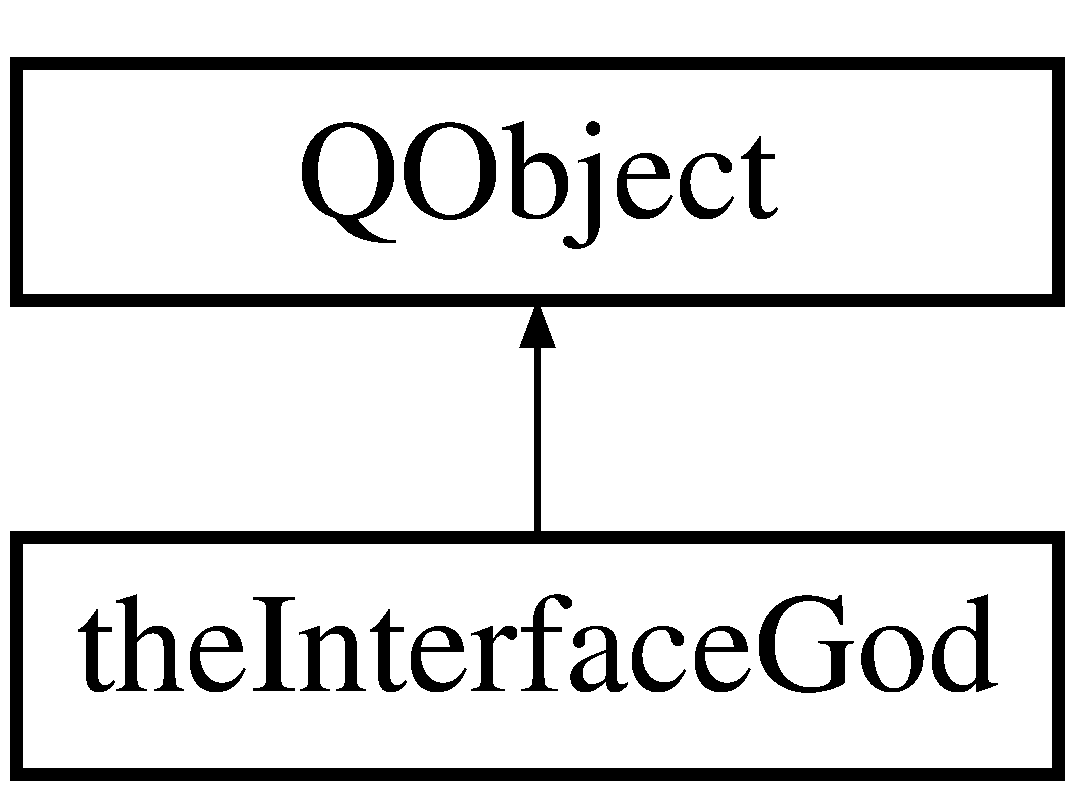
\includegraphics[height=2.000000cm]{classthe_interface_god}
\end{center}
\end{figure}
\subsection*{Signals}
\begin{DoxyCompactItemize}
\item 
\mbox{\Hypertarget{classthe_interface_god_a2d28c5450fc8a834749171a0548055e0}\label{classthe_interface_god_a2d28c5450fc8a834749171a0548055e0}} 
void {\bfseries S\+I\+G\+\_\+regenerate\+Frame\+List} (const int \&duration, const int \&frame\+Duration)
\item 
\mbox{\Hypertarget{classthe_interface_god_a84053294d490359ad575429be4cc6240}\label{classthe_interface_god_a84053294d490359ad575429be4cc6240}} 
void {\bfseries S\+I\+G\+\_\+play\+Frame} (const int \&frame\+No)
\end{DoxyCompactItemize}
\subsection*{Public Member Functions}
\begin{DoxyCompactItemize}
\item 
\mbox{\Hypertarget{classthe_interface_god_aa59f4c4386a001ae457caec3be6c3f8b}\label{classthe_interface_god_aa59f4c4386a001ae457caec3be6c3f8b}} 
{\bfseries the\+Interface\+God} (Q\+Object $\ast$parent=nullptr)
\item 
\mbox{\Hypertarget{classthe_interface_god_ab09c9557161f6ddd4fd7aba98df84452}\label{classthe_interface_god_ab09c9557161f6ddd4fd7aba98df84452}} 
Q\+\_\+\+I\+N\+V\+O\+K\+A\+B\+LE void {\bfseries regenerate\+Frame\+List} (const int \&duration, const int \&frame\+Duration)
\item 
\mbox{\Hypertarget{classthe_interface_god_a6e96d3eaf1f4589f05177f531df54ffe}\label{classthe_interface_god_a6e96d3eaf1f4589f05177f531df54ffe}} 
Q\+\_\+\+I\+N\+V\+O\+K\+A\+B\+LE void {\bfseries play\+Frame} (const int \&frame\+No)
\end{DoxyCompactItemize}


\subsection{Detailed Description}


Definition at line 6 of file theinterfacegod.\+h.



The documentation for this class was generated from the following files\+:\begin{DoxyCompactItemize}
\item 
theinterfacegod.\+h\item 
debug/moc\+\_\+theinterfacegod.\+cpp\item 
theinterfacegod.\+cpp\end{DoxyCompactItemize}

\hypertarget{classtime_slot}{}\section{time\+Slot Class Reference}
\label{classtime_slot}\index{time\+Slot@{time\+Slot}}


\subsection{Detailed Description}


Definition at line 8 of file timeslot.\+h.



The documentation for this class was generated from the following file\+:\begin{DoxyCompactItemize}
\item 
timeslot.\+h\end{DoxyCompactItemize}

\hypertarget{structtime_slot_item}{}\section{time\+Slot\+Item Struct Reference}
\label{structtime_slot_item}\index{time\+Slot\+Item@{time\+Slot\+Item}}
\subsection*{Public Attributes}
\begin{DoxyCompactItemize}
\item 
\mbox{\Hypertarget{structtime_slot_item_ab430dbd2e7c46c9bd87554d8e3bbaf64}\label{structtime_slot_item_ab430dbd2e7c46c9bd87554d8e3bbaf64}} 
int {\bfseries id}
\item 
\mbox{\Hypertarget{structtime_slot_item_aadbe53740fe10b76311f689694089b1f}\label{structtime_slot_item_aadbe53740fe10b76311f689694089b1f}} 
int {\bfseries from\+Ms}
\item 
\mbox{\Hypertarget{structtime_slot_item_a4b74d22205b5f6c22e6d0f18f2c42d6e}\label{structtime_slot_item_a4b74d22205b5f6c22e6d0f18f2c42d6e}} 
int {\bfseries to\+Ms}
\item 
\mbox{\Hypertarget{structtime_slot_item_ab5b1e73d9a3dba3e043d23ad807653e6}\label{structtime_slot_item_ab5b1e73d9a3dba3e043d23ad807653e6}} 
quint8 {\bfseries group}
\item 
\mbox{\Hypertarget{structtime_slot_item_a4f805f461449412752fbebc567e6bcca}\label{structtime_slot_item_a4f805f461449412752fbebc567e6bcca}} 
bool {\bfseries Valve\+On\+Off}
\item 
\mbox{\Hypertarget{structtime_slot_item_ae5237412d9e862b0b9b98b55c6617dd7}\label{structtime_slot_item_ae5237412d9e862b0b9b98b55c6617dd7}} 
bool {\bfseries Led\+On\+Off}
\item 
\mbox{\Hypertarget{structtime_slot_item_a6a3286dc5c1dfa1af679f1ab550a0e3a}\label{structtime_slot_item_a6a3286dc5c1dfa1af679f1ab550a0e3a}} 
bool {\bfseries Inverter}
\item 
\mbox{\Hypertarget{structtime_slot_item_af23116ebe70f2174eb22eb18a667ff1b}\label{structtime_slot_item_af23116ebe70f2174eb22eb18a667ff1b}} 
quint8 {\bfseries Led\+Mode}
\item 
\mbox{\Hypertarget{structtime_slot_item_a50752f5574513d60caf9c19e4cb3d71b}\label{structtime_slot_item_a50752f5574513d60caf9c19e4cb3d71b}} 
quint8 {\bfseries Inverter\+Level}
\item 
\mbox{\Hypertarget{structtime_slot_item_a6d29e12d908b61c958164feabeb2f7f3}\label{structtime_slot_item_a6d29e12d908b61c958164feabeb2f7f3}} 
Q\+String {\bfseries file\+Bin\+Path}
\item 
\mbox{\Hypertarget{structtime_slot_item_ad89dc59d6c1e3a9e6bccfd73f08749b3}\label{structtime_slot_item_ad89dc59d6c1e3a9e6bccfd73f08749b3}} 
Q\+String {\bfseries Led\+Values\+List}
\item 
\mbox{\Hypertarget{structtime_slot_item_aa4e617582e427c315d09c5c7b36db8d6}\label{structtime_slot_item_aa4e617582e427c315d09c5c7b36db8d6}} 
quint8 {\bfseries Led\+Channels}
\item 
\mbox{\Hypertarget{structtime_slot_item_a54c7fe8430f5a93444f6ade27d78a18d}\label{structtime_slot_item_a54c7fe8430f5a93444f6ade27d78a18d}} 
quint8 {\bfseries Valve\+Channels}
\item 
\mbox{\Hypertarget{structtime_slot_item_a6d46f1f32495c6a9b186cd775d095ba1}\label{structtime_slot_item_a6d46f1f32495c6a9b186cd775d095ba1}} 
quint8 {\bfseries Valve\+Mode}
\end{DoxyCompactItemize}


\subsection{Detailed Description}


Definition at line 7 of file timeslotlist.\+h.



The documentation for this struct was generated from the following file\+:\begin{DoxyCompactItemize}
\item 
timeslotlist.\+h\end{DoxyCompactItemize}

\hypertarget{classtime_slot_list}{}\section{time\+Slot\+List Class Reference}
\label{classtime_slot_list}\index{time\+Slot\+List@{time\+Slot\+List}}
Inheritance diagram for time\+Slot\+List\+:\begin{figure}[H]
\begin{center}
\leavevmode
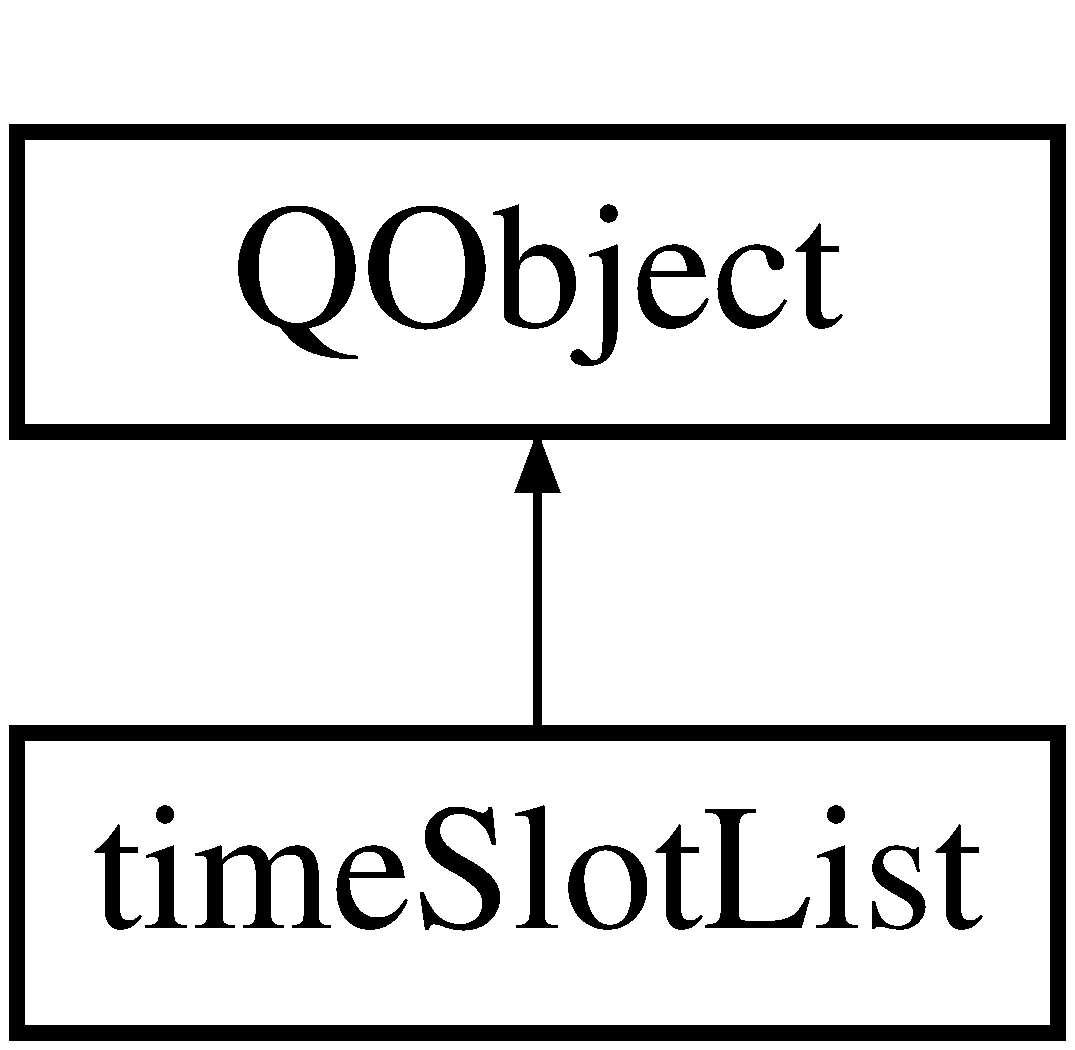
\includegraphics[height=2.000000cm]{classtime_slot_list}
\end{center}
\end{figure}
\subsection*{Public Slots}
\begin{DoxyCompactItemize}
\item 
\mbox{\Hypertarget{classtime_slot_list_a6f8f70ee657d26a777f278d778ba4175}\label{classtime_slot_list_a6f8f70ee657d26a777f278d778ba4175}} 
void {\bfseries append\+Item} (const quint8 \&group, const int \&from\+Ms, const int \&to\+Ms)
\item 
\mbox{\Hypertarget{classtime_slot_list_aff5f7a216fd8e4d2a17066c4ba42093d}\label{classtime_slot_list_aff5f7a216fd8e4d2a17066c4ba42093d}} 
void {\bfseries remove\+Items} (const int \&id)
\end{DoxyCompactItemize}
\subsection*{Signals}
\begin{DoxyCompactItemize}
\item 
\mbox{\Hypertarget{classtime_slot_list_a10230e14b11a55c793dd50787bf3d300}\label{classtime_slot_list_a10230e14b11a55c793dd50787bf3d300}} 
void {\bfseries pre\+Item\+Appended} ()
\item 
\mbox{\Hypertarget{classtime_slot_list_a6fb04319700b8efb24d173ee58b07945}\label{classtime_slot_list_a6fb04319700b8efb24d173ee58b07945}} 
void {\bfseries post\+Item\+Appended} ()
\item 
\mbox{\Hypertarget{classtime_slot_list_a7083a0f925da9af04d17e11fdc35ea47}\label{classtime_slot_list_a7083a0f925da9af04d17e11fdc35ea47}} 
void {\bfseries pre\+Item\+Removed} (int index)
\item 
\mbox{\Hypertarget{classtime_slot_list_a220054e6bd363e699cd7ca2209d861ba}\label{classtime_slot_list_a220054e6bd363e699cd7ca2209d861ba}} 
void {\bfseries post\+Item\+Removed} ()
\item 
\mbox{\Hypertarget{classtime_slot_list_ab929a81211c334bd61600741b0d99ffa}\label{classtime_slot_list_ab929a81211c334bd61600741b0d99ffa}} 
void {\bfseries time\+Slot\+Item\+Changed} (const \mbox{\hyperlink{structtime_slot_item}{time\+Slot\+Item}} \&item)
\item 
\mbox{\Hypertarget{classtime_slot_list_a5ec2f91f9a292545664d3d4b97e21770}\label{classtime_slot_list_a5ec2f91f9a292545664d3d4b97e21770}} 
void {\bfseries time\+Slot\+Item\+Removed} (const \mbox{\hyperlink{structtime_slot_item}{time\+Slot\+Item}} \&item)
\end{DoxyCompactItemize}
\subsection*{Public Member Functions}
\begin{DoxyCompactItemize}
\item 
\mbox{\Hypertarget{classtime_slot_list_a1cd9b1ac08dba361f5559e686e74e6fd}\label{classtime_slot_list_a1cd9b1ac08dba361f5559e686e74e6fd}} 
{\bfseries time\+Slot\+List} (Q\+Object $\ast$parent=nullptr)
\item 
\mbox{\Hypertarget{classtime_slot_list_ae4c1727831d22818a99ee50d21378b82}\label{classtime_slot_list_ae4c1727831d22818a99ee50d21378b82}} 
Q\+Vector$<$ \mbox{\hyperlink{structtime_slot_item}{time\+Slot\+Item}} $>$ {\bfseries items} () const
\item 
\mbox{\Hypertarget{classtime_slot_list_a31647cc65b8a4ba56516b5ae4df84dac}\label{classtime_slot_list_a31647cc65b8a4ba56516b5ae4df84dac}} 
bool {\bfseries set\+Item\+At} (int index, const \mbox{\hyperlink{structtime_slot_item}{time\+Slot\+Item}} \&item)
\item 
\mbox{\Hypertarget{classtime_slot_list_a06f8f6e6f14c14c88e3bb1ded2f456c4}\label{classtime_slot_list_a06f8f6e6f14c14c88e3bb1ded2f456c4}} 
Q\+\_\+\+I\+N\+V\+O\+K\+A\+B\+LE int {\bfseries time\+Slot\+Collision\+Check} (const int \&id)
\item 
\mbox{\Hypertarget{classtime_slot_list_a33b47cc51453492e0e6fab1266c6bca7}\label{classtime_slot_list_a33b47cc51453492e0e6fab1266c6bca7}} 
Q\+\_\+\+I\+N\+V\+O\+K\+A\+B\+LE bool {\bfseries get\+Collision\+Side} ()
\item 
\mbox{\Hypertarget{classtime_slot_list_a2bfee5da3e54d9e737ba28ad8d15aca4}\label{classtime_slot_list_a2bfee5da3e54d9e737ba28ad8d15aca4}} 
Q\+\_\+\+I\+N\+V\+O\+K\+A\+B\+LE int {\bfseries count} ()
\item 
\mbox{\Hypertarget{classtime_slot_list_aac922a60e02bcd55751cdce7319d0233}\label{classtime_slot_list_aac922a60e02bcd55751cdce7319d0233}} 
Q\+\_\+\+I\+N\+V\+O\+K\+A\+B\+LE int {\bfseries last\+Index} () const
\end{DoxyCompactItemize}
\subsection*{Public Attributes}
\begin{DoxyCompactItemize}
\item 
\mbox{\Hypertarget{classtime_slot_list_a55069a5cdebfd5e4dfca2ee72ebb11a3}\label{classtime_slot_list_a55069a5cdebfd5e4dfca2ee72ebb11a3}} 
int {\bfseries m\+Group}
\end{DoxyCompactItemize}


\subsection{Detailed Description}


Definition at line 39 of file timeslotlist.\+h.



The documentation for this class was generated from the following files\+:\begin{DoxyCompactItemize}
\item 
timeslotlist.\+h\item 
debug/moc\+\_\+timeslotlist.\+cpp\item 
timeslotlist.\+cpp\end{DoxyCompactItemize}

\hypertarget{classtime_slot_model}{}\section{time\+Slot\+Model Class Reference}
\label{classtime_slot_model}\index{time\+Slot\+Model@{time\+Slot\+Model}}
Inheritance diagram for time\+Slot\+Model\+:\begin{figure}[H]
\begin{center}
\leavevmode
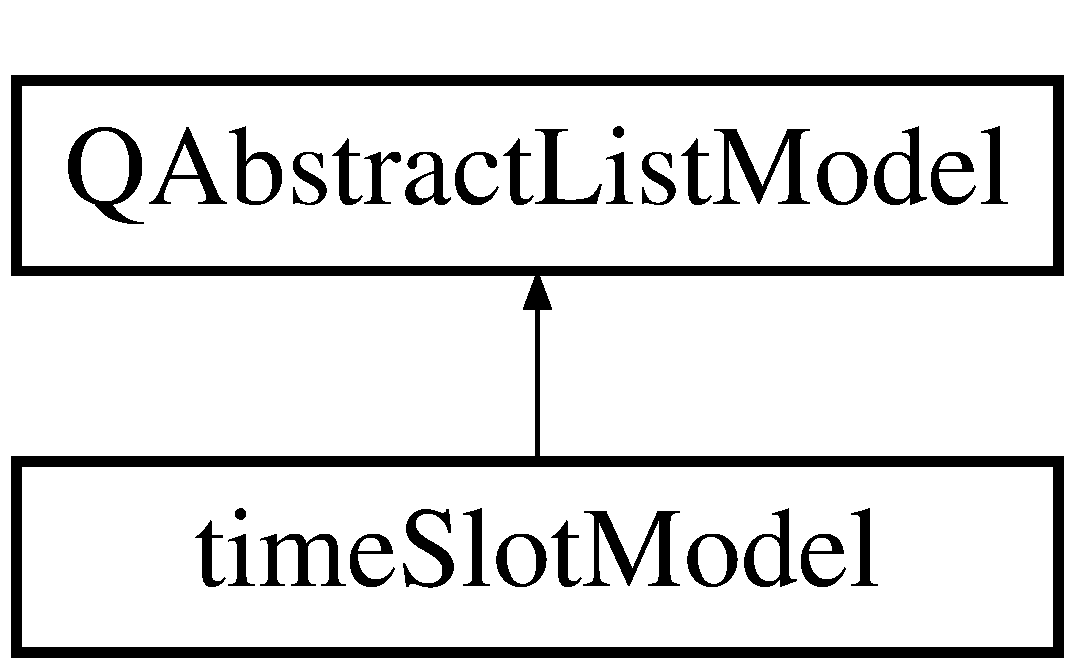
\includegraphics[height=2.000000cm]{classtime_slot_model}
\end{center}
\end{figure}
\subsection*{Public Types}
\begin{DoxyCompactItemize}
\item 
\mbox{\Hypertarget{classtime_slot_model_a5c2509a4c20e6cbafb13d582c2e73424}\label{classtime_slot_model_a5c2509a4c20e6cbafb13d582c2e73424}} 
enum \{ \newline
{\bfseries I\+D\+Role} = Qt\+:\+:User\+Role, 
{\bfseries Group\+Role}, 
{\bfseries Valve\+On\+Off\+Role}, 
{\bfseries Led\+On\+Off\+Role}, 
\newline
{\bfseries Inverter\+Role}, 
{\bfseries From\+Ms\+Role}, 
{\bfseries To\+Ms\+Role}, 
{\bfseries Led\+Mode\+Role}, 
\newline
{\bfseries Inverter\+Level\+Role}, 
{\bfseries File\+Bin\+Path\+Role}, 
{\bfseries L\+E\+D\+Values\+List\+Role}, 
{\bfseries L\+E\+D\+Channels\+Role}, 
\newline
{\bfseries Valve\+Channels\+Role}, 
{\bfseries Valve\+Mode\+Role}
 \}
\end{DoxyCompactItemize}
\subsection*{Signals}
\begin{DoxyCompactItemize}
\item 
\mbox{\Hypertarget{classtime_slot_model_a76b7beaf6bf598a5e12cf0e57100ffd1}\label{classtime_slot_model_a76b7beaf6bf598a5e12cf0e57100ffd1}} 
void {\bfseries size\+Changed} ()
\end{DoxyCompactItemize}
\subsection*{Public Member Functions}
\begin{DoxyCompactItemize}
\item 
\mbox{\Hypertarget{classtime_slot_model_a24787c0ad1a00e00d11542c019802576}\label{classtime_slot_model_a24787c0ad1a00e00d11542c019802576}} 
{\bfseries time\+Slot\+Model} (Q\+Object $\ast$parent=nullptr)
\item 
\mbox{\Hypertarget{classtime_slot_model_adbccd19c8555413b2c45005d4ab4eac5}\label{classtime_slot_model_adbccd19c8555413b2c45005d4ab4eac5}} 
int {\bfseries row\+Count} (const Q\+Model\+Index \&parent=Q\+Model\+Index()) const override
\item 
\mbox{\Hypertarget{classtime_slot_model_ab3f9a4d41419bc39d0d516332a45c001}\label{classtime_slot_model_ab3f9a4d41419bc39d0d516332a45c001}} 
Q\+Variant {\bfseries data} (const Q\+Model\+Index \&index, int role=Qt\+::\+Display\+Role) const override
\item 
\mbox{\Hypertarget{classtime_slot_model_a9b4e404c24a5580a317661a3f0b9b62e}\label{classtime_slot_model_a9b4e404c24a5580a317661a3f0b9b62e}} 
bool {\bfseries set\+Data} (const Q\+Model\+Index \&index, const Q\+Variant \&value, int role=Qt\+::\+Edit\+Role) override
\item 
\mbox{\Hypertarget{classtime_slot_model_a116236ac7f08d69a7f5f841b959dca6a}\label{classtime_slot_model_a116236ac7f08d69a7f5f841b959dca6a}} 
Qt\+::\+Item\+Flags {\bfseries flags} (const Q\+Model\+Index \&index) const override
\item 
\mbox{\Hypertarget{classtime_slot_model_ab37cf6b39ebb3e3fc77e96c0371f26ea}\label{classtime_slot_model_ab37cf6b39ebb3e3fc77e96c0371f26ea}} 
Q\+\_\+\+I\+N\+V\+O\+K\+A\+B\+LE Q\+Variant {\bfseries get\+Data\+Per\+Index} (const int \&index, const Q\+Byte\+Array \&Role\+String)
\item 
\mbox{\Hypertarget{classtime_slot_model_ad5685549c714bca4da318d4dc12f1ca2}\label{classtime_slot_model_ad5685549c714bca4da318d4dc12f1ca2}} 
Q\+\_\+\+I\+N\+V\+O\+K\+A\+B\+LE bool {\bfseries set\+Data\+Per\+Index} (const int \&index, const Q\+Byte\+Array \&Role\+String, const Q\+Variant \&value)
\item 
\mbox{\Hypertarget{classtime_slot_model_aec577d91ac6373d6f5b52f82a3fce0bb}\label{classtime_slot_model_aec577d91ac6373d6f5b52f82a3fce0bb}} 
virtual Q\+Hash$<$ int, Q\+Byte\+Array $>$ {\bfseries role\+Names} () const override
\item 
\mbox{\Hypertarget{classtime_slot_model_a545f2f51bc855c04e4f47964fc79ca19}\label{classtime_slot_model_a545f2f51bc855c04e4f47964fc79ca19}} 
\mbox{\hyperlink{classtime_slot_list}{time\+Slot\+List}} $\ast$ {\bfseries list} () const
\item 
\mbox{\Hypertarget{classtime_slot_model_a59aa5f346460a6aaef9b2b196e61cedc}\label{classtime_slot_model_a59aa5f346460a6aaef9b2b196e61cedc}} 
void {\bfseries set\+List} (\mbox{\hyperlink{classtime_slot_list}{time\+Slot\+List}} $\ast$list)
\item 
\mbox{\Hypertarget{classtime_slot_model_a974ad7212eee6066625c7ad37f628210}\label{classtime_slot_model_a974ad7212eee6066625c7ad37f628210}} 
int {\bfseries size} () const
\item 
\mbox{\Hypertarget{classtime_slot_model_a826b092b7df775286882ba7f9cee82db}\label{classtime_slot_model_a826b092b7df775286882ba7f9cee82db}} 
void {\bfseries set\+Size} (int size)
\end{DoxyCompactItemize}
\subsection*{Properties}
\begin{DoxyCompactItemize}
\item 
\mbox{\Hypertarget{classtime_slot_model_a330c04e7bfd74add76d8d3dbf7da6e30}\label{classtime_slot_model_a330c04e7bfd74add76d8d3dbf7da6e30}} 
\mbox{\hyperlink{classtime_slot_list}{time\+Slot\+List}} {\bfseries list}
\item 
\mbox{\Hypertarget{classtime_slot_model_a04b118aa0a283bc1441eb1d3da649438}\label{classtime_slot_model_a04b118aa0a283bc1441eb1d3da649438}} 
int {\bfseries size}
\end{DoxyCompactItemize}


\subsection{Detailed Description}


Definition at line 7 of file timeslotmodel.\+h.



The documentation for this class was generated from the following files\+:\begin{DoxyCompactItemize}
\item 
timeslotmodel.\+h\item 
debug/moc\+\_\+timeslotmodel.\+cpp\item 
timeslotmodel.\+cpp\end{DoxyCompactItemize}

%--- End generated contents ---

% Index
\backmatter
\newpage
\phantomsection
\clearemptydoublepage
\addcontentsline{toc}{chapter}{Index}
\printindex

\end{document}
